Metody sdílení přenosového kanálu se dělí na:
\begin{itemize}
	\item \textbf{deterministické} (bezkolizní) -- řídí se algoritmem, který přesně definuje kdo, kdy bude vysílat a ke kolizím nedochází.
	\item \textbf{nedeterministické} (kolizní) -- algoritmus je založen na náhodě (náhodné časové prodlevy) a musí řešit kolize (situace, kdy chce naráz na kanálu vysílat více stanic)
\end{itemize}

\subsection{Bezkolizní (deterministické) metody sdílení média}
Deterministické metody se dělí na -- \textbf{Centralizované řízení} a \textbf{Distribuované řízení}

\subsubsection{Centralizované řízení}
Jedna ze stanic je \textbf{master} a přiděluje ostatním právo vysílat. \textbf{Efektivní}, ale část kanálu použita pro komunikaci s masterem.
\begin{itemize}
	\item \textbf{Přidělování na výzvu} - nejstarší, původně v terminálových systémech nad protokoly BSC a HDLC. Stanice smí vysílat jen, když je k tomu vyzvána masterem.
	\begin{itemize}
	\item \textbf{Cyklická výzva} - vyzývaná stanice \textbf{buď vyšle rámec, nebo odmítne výzvu}, příp. neodpoví. Použitelné pro \textbf{malé zpoždění} na kanále. Rozumné pro vysoké využití kanálu. Pro malé zatížení a velký počet stanic neefektivní.
	\item \textbf{Binární vyhledávání} - pro kanál, u kterého může stanice rozpoznat,\textbf{ zda vysílá jedna nebo více stanic}. Při malém zatížení a velkém počtu stanic je efektivní vyhledávat stanici připravenou vysílat binárním vyhledáváním. Stanice se zorganizují do stromu podle jednotlivých bitů adres, řídící stanice postupně vyzývá skupiny stanic, aktivní stanice ve vyzvané skupině odpoví signálem na sdíleném kanále. Pokud stanice zjistí, že je jediná, která odpovídá, může začít vysílat, jinak se výzva posune o jednu úroveň dolů ve stromu. \textbf{Rychlejší pro malé zátěže.}
\end{itemize}
	\item \textbf{Přidělování na žádost} - žádosti od stanic přicházejí k řídící stanici po \textbf{vyhrazených kanálech}, vyhrazených kanálů se v klasických počítačových sítích LAN/WAN prakticky nepoužívá, spíše u sběrnic počítačů. Použití možné i v rádiových sítích, využití vyhrazeného \textbf{nízkorychlostního} podkanálu časového multiplexu.
\end{itemize}

\subsubsection{Distribuované řízení}
Nezávislé na řídící stanici.
\begin{itemize}
	\item \textbf{Rezervace kanálu} - rezervační rámec, ve svém slotu může každá stanice \textbf{požádat o přidělení slotu} v datovém kanále, datové sloty následují podle okamžitého požadovaného počtu za rezervačním rámcem. \textbf{Neefektivní pro velký počet stanic} na rozlehlé síti s malou zátěží. Na prázdném kanále neustálé opakování rezervačních slotů.
	\begin{figure}[H]
		\centering
		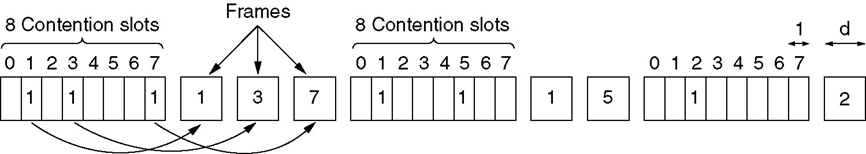
\includegraphics[width=0.8\textwidth]{assets/rezervace_kanalu}
	\end{figure}
	\item \textbf{Binární vyhledávání} -  stanice nejprve postupně vysílají bity své adresy od nejvyššího řádu, na sběrnici se logicky sčítají [OR]. Jakmile \textbf{stanice vysílá 0 a čte 1}, chce vysílat někdo s vyšší prioritou a stanice musí \textbf{zmlknout}.
	\begin{figure}[H]
		\centering
		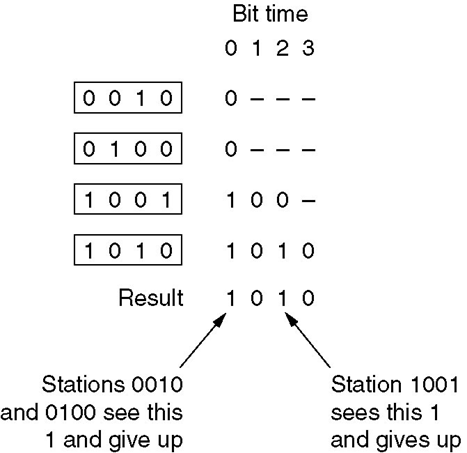
\includegraphics[width=0.4\textwidth]{assets/binarni_vyhledavani}
	\end{figure}
	\item \textbf{Logický kruh [Token Passing Bus]} - adresy stanic tvoří cyklickou posloupnost, každá stanice zná svou adresu a adresu následníka. Mezi stanicemi se cyklicky předává právo k vysílání (token). Stanice vlastnící token smí vysílat, do určité doby však musí předat token následníkovi. Problém počátečního ustavení posloupnosti, odpojování a připojování stanic do logického kruhu za provozu (rekonfigurace). Velké zpoždění při malé zátěži a velkém počtu stanic.
	\item \textbf{Virtuální logický kruh} - po odvysílání rámce je každý další stanici vyhrazen \textbf{časový interval}, kdy smí začít vysílat, nevyužije-li jej, následuje interval další stanice. Nutnost synchronizace stanic. V oblasti malých zátěží efektivnější než logický kruh.
\end{itemize}

\subsection{Kolizní (nedeterministické) metody sdílení média}
\subsubsection{Aloha}
Původně na rádiové síti univerzity na Havajských ostrovech. \textbf{Netestuje se obsazenost média}, dodnes použití pro rádiové a družicové sítě, kde velké zpoždění signálu nebo konstrukce anténních obvodů zamezují příposlechu vlastního vysílání.

\begin{itemize}
	\item \textbf{Prostá Aloha}
\begin{itemize}
\item Stanice \textbf{vysílají bez ohledu na cokoliv}.
\item \textbf{Časový limit pro potvrzení}, při vypršení náhodné pozdržení (aby nedošlo k opakované kolizi) a opakování pokusu.
\item \textbf{Kolizní slot}: \textbf{2*t0} [t0-doba pro vyslání rámce]. \textbf{Dvojnásobek}, protože může být zarušen koncem jiného rámce. Kolizní slot udává, kolik času se nejvýše ztratí na nevyužití kanálu vlivem kolize. 
\end{itemize}

\item \textbf{Taktovaná Aloha}
\begin{itemize}
\item Vysílat se smí začít jen v okamžicích začátků \textbf{časových úseků} pro odeslání jednoho rámce.
\item \textbf{Kolizní slot} je \textbf{poloviční} než u prosté Alohy.
\item \textbf{Exponenciální závislost}, malý vzrůst zátěže může významně zvýšit počet opakování a snížit průchodnost kanálu.
\end{itemize}

\item \textbf{Řízená Aloha}
\begin{itemize}
\item \textbf{Řízená změna intenzity opakování} podle stavu sítě: vyšší intenzita opakování => rychlejší předání rámce, při blížícími se zablokování se intenzita sníží.
\item \textbf{Případně sledování provozu na kanále} [poměru neobsazených slotů] a nastavování intenzity.
\end{itemize}
\end{itemize}

\subsubsection{Carrier Sense Multiple Access (CSMA)}
Skupina metod \textbf{náhodného přístupu s příposlechem nosné}, tj. využití znalosti o obsazení kanálu. Podmínky pro aplikaci: \textbf{dokonalá slyšitelnost stanic}, \textbf{malé zpoždění signálu} (což platí v LAN).

\begin{enumerate}
\item \textbf{CSMA (naléhanící CSMA, 1-persistant CSMA)} -- před odesláním rámce se testuje stav kanálu, je-li obsazen, odloží se vysílání na okamžik jeho uvolnění. Riziko kolize stanic čekajících na uvolnění kanálu. Při obsazení kanálu čekání náhodnou dobu před dalším pokusem.
\item \textbf{Nenaléhající CSMA (non-persistant CSMA)} -- při detekci obsazeného kanálu se počká náhodnou dobu pak opět test obsazení. Čekací doba se obvykle volí jako k-násobek doby průchodu signálu sběrnicí.
\item \textbf{P-naléhající CSMA (p-persistant CSMA)} -- při obsazení kanálu v okamžiku potřeby vysílání se počká na uvolnění kanálu (nebo byl volný okamžitě), pak se \textbf{s pravdě podobností p} začne vysílat, s pravděpodobností (1-p) se počká krátký interval, pak se opakuje do úspěšného odeslání rámce. Volbou p lze nastavit optimální využití kanálu pro danou zátěž. Pro p=1 jde o naléhající CSMA.
\end{enumerate}

\begin{figure}[H]
	\centering
	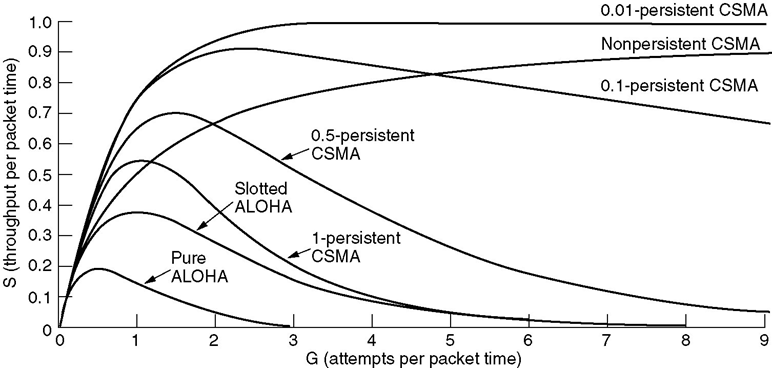
\includegraphics[width=0.62\textwidth]{assets/csma-grafy}
\end{figure}

\subsubsection{Carrier Sense Multiple Access with Collision Detection (CSMA/CD)}
\begin{itemize}
\item CSMA \textbf{s detekcí kolize} (sledování vlastního vysílání).
\item Využívá se u klasického \textbf{Ethernetu}.
\item Před vysíláním musí být na médiu klid po dobu kolizního slotu.
\item Jinak postup odpovídá naléhající CSMA.
\item \textbf{Okamžité ukončení vysílání po detekci kolize} - kanál se zbytečně nezaplňuje rámcem, který je stejně zkolidován.
\item Závislost maximální délky segmentu na \textbf{rychlosti šíření signálu} (vztah s dobou vysílání rámce a minimální délkou rámce)
\item Nutnost kódování, které \textbf{umožňují detekci kolize} (otevřený kolektor, měření napětí na médiu generovaného proudovými zdroji vysílačů).
\item Při \textbf{detekci kolize stanice }vysílá kolizní signál [\textbf{jam}], aby kolizi rozpoznaly všechny kolidující stanice. O opakování se stanice pokusí až po náhodné časové prodlevě, stabilitu metody nutno zajistit řízením intenzity opakování.
\end{itemize}

\begin{figure}[H]
	\centering
	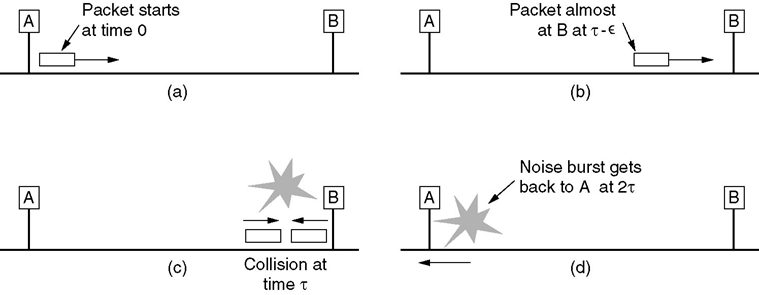
\includegraphics[width=0.62\textwidth]{assets/csma-cd-casovani_kolize}
\end{figure}

\subsubsection{Carrier Sense Multiple Access with Collision Avoidance (CSMA/CA)}
\textbf{Rezervace intervalu} po odvysílání rámce pro potvrzení (v předchozích metodách jsme na potvrzení nahlíželi jako na  přídavnou zátěž). Před začátkem vysílání paketu stanice určitý čas poslouchá, zda je přenosové médium volné. Pokud ano, oznámí vysílání a rezervuje přenosové médium a může zahájit vysílání. V opačném případě čeká na konec právě probíhajícího vysílání. Využití v \textbf{Wi-Fi}.
